\subsection{Solución actividad 2}
%\begin{center}
%	\csvautotabular{latex/tablactividad2.csv}
%\end{center}
2. Coloque en el código en simulink una entrada tipo step con un valor inicial 0[u], un valor final 5[u] y un tiempo de desfasamiento de 0[s], observe y analice la respuesta obtenida en el osciloscopio.\\

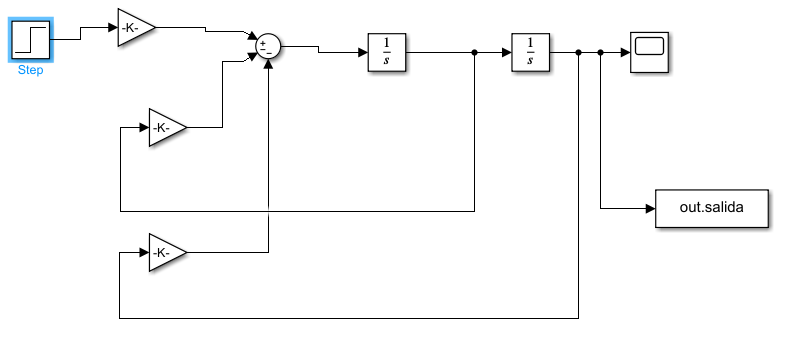
\includegraphics[scale=0.6]{actividad2Circuito.png}

3. Variar el parámetro $R_1$ del sistema representado por la Fig. (38) con el objetivo de encontrar las diferentes respuestas a escalón del sistema de segundo orden representado por la Ecuación (40) y registre sus resultados en la tabla.\\
\begin{center}
	\begin{tabular}{ |c|c|c|c|c| }
		\hline
		Tipo de respuesta & Capacitor & Inductor & $Resistencia_{min}$ & $Resistencia_{max}$\\
		\hline
		No amortiguada & 4.4$\mu F$ & 0.05$Hz$ & 0$\Omega$ & 0$\Omega$\\
		\hline
		Subamortiguada & 0.22$\mu F$ & 0.05$Hz$ & 100$\Omega$ & 900$\Omega$\\
		\hline
		Críticamente amortiguada & 0.22$\mu F$ & 0.05$Hz$ & 1000$\Omega$ & 5000$\Omega$\\
		\hline
		Sobreamortiguada & 4.4$\mu F$ & 0.05$Hz$ & 2000$\Omega$ & 5000$\Omega$\\
		\hline
	\end{tabular}
\end{center}
4. ¿En un sistema real se podrían obtener los cuatro tipos de respuesta? Justifique su respuesta.\\
No es posible obtener los cuatro comportamientos. Las respuestas al escalón del sistema de segundo orden dependen de $\zeta$ y para obtener el comportamiento no amortiguado necesitamos la siguiente condición: $\zeta=0$ lo cual no se puede obtener con nuestro circuito eléctrico. Debido a la naturaleza del diseño de nuestro circuito necesitamos de una resistencia de $0\Omega$ o que tienda a $0\Omega$ para obtener el comportamiento del caso en que es no amortiguado o una capacitancia de $0F$ para obtener dicha respuesta, lo cual no es posible.\\

